% -*- eval: (load-file "./autoloader.el")  -*-

\documentclass[25pt, a0paper, portrait]{tikzposter}
\title{\parbox{\linewidth}{\centering Transparently Using Non-Volatile Memory with Taenite, A Rust Transactional NVM Library}}
\author{Louis Boulanger, Frédéric Wagner, Yves Denneulin}
\institute{Univ. Grenoble Alpes, CNRS, Inria, Grenoble INP, LIG}

\usetikzlibrary{arrows, arrows.meta, decorations.pathreplacing}
\usepackage{lmodern}
\usepackage{minted}

% Arial-like font, Helvetica
\usepackage{helvet}
\renewcommand\familydefault{\sfdefault}


% \Huge isn't enough. First argument to \fontsize is the size, second is spacing (should be 1.2x font size)
\newcommand*{\HUGE}{\fontsize{80}{96}\selectfont}

% Color palette and style
\definecolorstyle{LIGStyle}{
  \definecolor{LIGBlue}{cmyk}{0.85,0.6,0.12,0}
  \definecolor{LIGLightBlue}{cmyk}{0.82,0.46,0,0}
  \definecolor{LIGGray}{cmyk}{0.64,0.54,0.52,0.52}
}{
  \colorlet{backgroundcolor}{white}
  \colorlet{framecolor}{white}
  \colorlet{titlefgcolor}{white}
  \colorlet{titlebgcolor}{LIGBlue}
  \colorlet{blocktitlebgcolor}{white}
  \colorlet{blocktitlefgcolor}{LIGBlue}
  \colorlet{blockbodybgcolor}{white}
  \colorlet{blockbodyfgcolor}{black}
}
\usecolorstyle{LIGStyle}

% Title style
\definetitlestyle{LIGTitle}{
  width=0.9\paperwidth, roundedcorners=0, 
}{
  \begin{scope}[line width=\titlelinewidth, rounded corners=\titleroundedcorners]
  \end{scope}
}

% Title format
\settitle{
  \vspace{-8mm}
  \centering\color{titlefgcolor}{\textbf{\HUGE \sffamily \@title}}
  
  {
    \vspace{30mm}
    \color{blockbodyfgcolor}{\LARGE \sffamily \@author \par}
    \vspace{1em}
    \color{blockbodyfgcolor}{\Large \sffamily \@institute \par}
  }
}

% Block style
\defineblockstyle{LIGBlock}{
  bodywidthscale=1
}{
  \ifBlockHasTitle
  \draw [line width=1mm] (blockbody.north west) -- (blockbody.north east);
  \fi
}

\usetitlestyle{LIGTitle}
\useblockstyle{LIGBlock}

\begin{document}
% Add LIG template png as background image
\node[above right,opacity=1,inner sep=0pt,outer sep=0pt] at (bottomleft) {\includegraphics[width=\paperwidth,height=\paperheight]{template}};

\maketitle

% Amazingly, tikzposter doesn't define "topleft" and "bottomright".
\coordinate (topleft)     at (topright -| bottomleft);
\coordinate (bottomright) at (topright |- bottomleft);

% Bar to separate authors from contents.
% Default tikz units are in cm, and A0 is 84.1cmx118.9cm. (0, 0) is the center of the page.
\draw[black, thick, line width=2mm, color=LIGBlue] (-42.05, 43) -- (42.05, 43);

\begin{columns}
  \column{0.5}
  \block{Why is NVRAM ``challenging'' to use?}{
    \begin{tikzfigure}[A memory hierarchy model including NVRAM\par]
      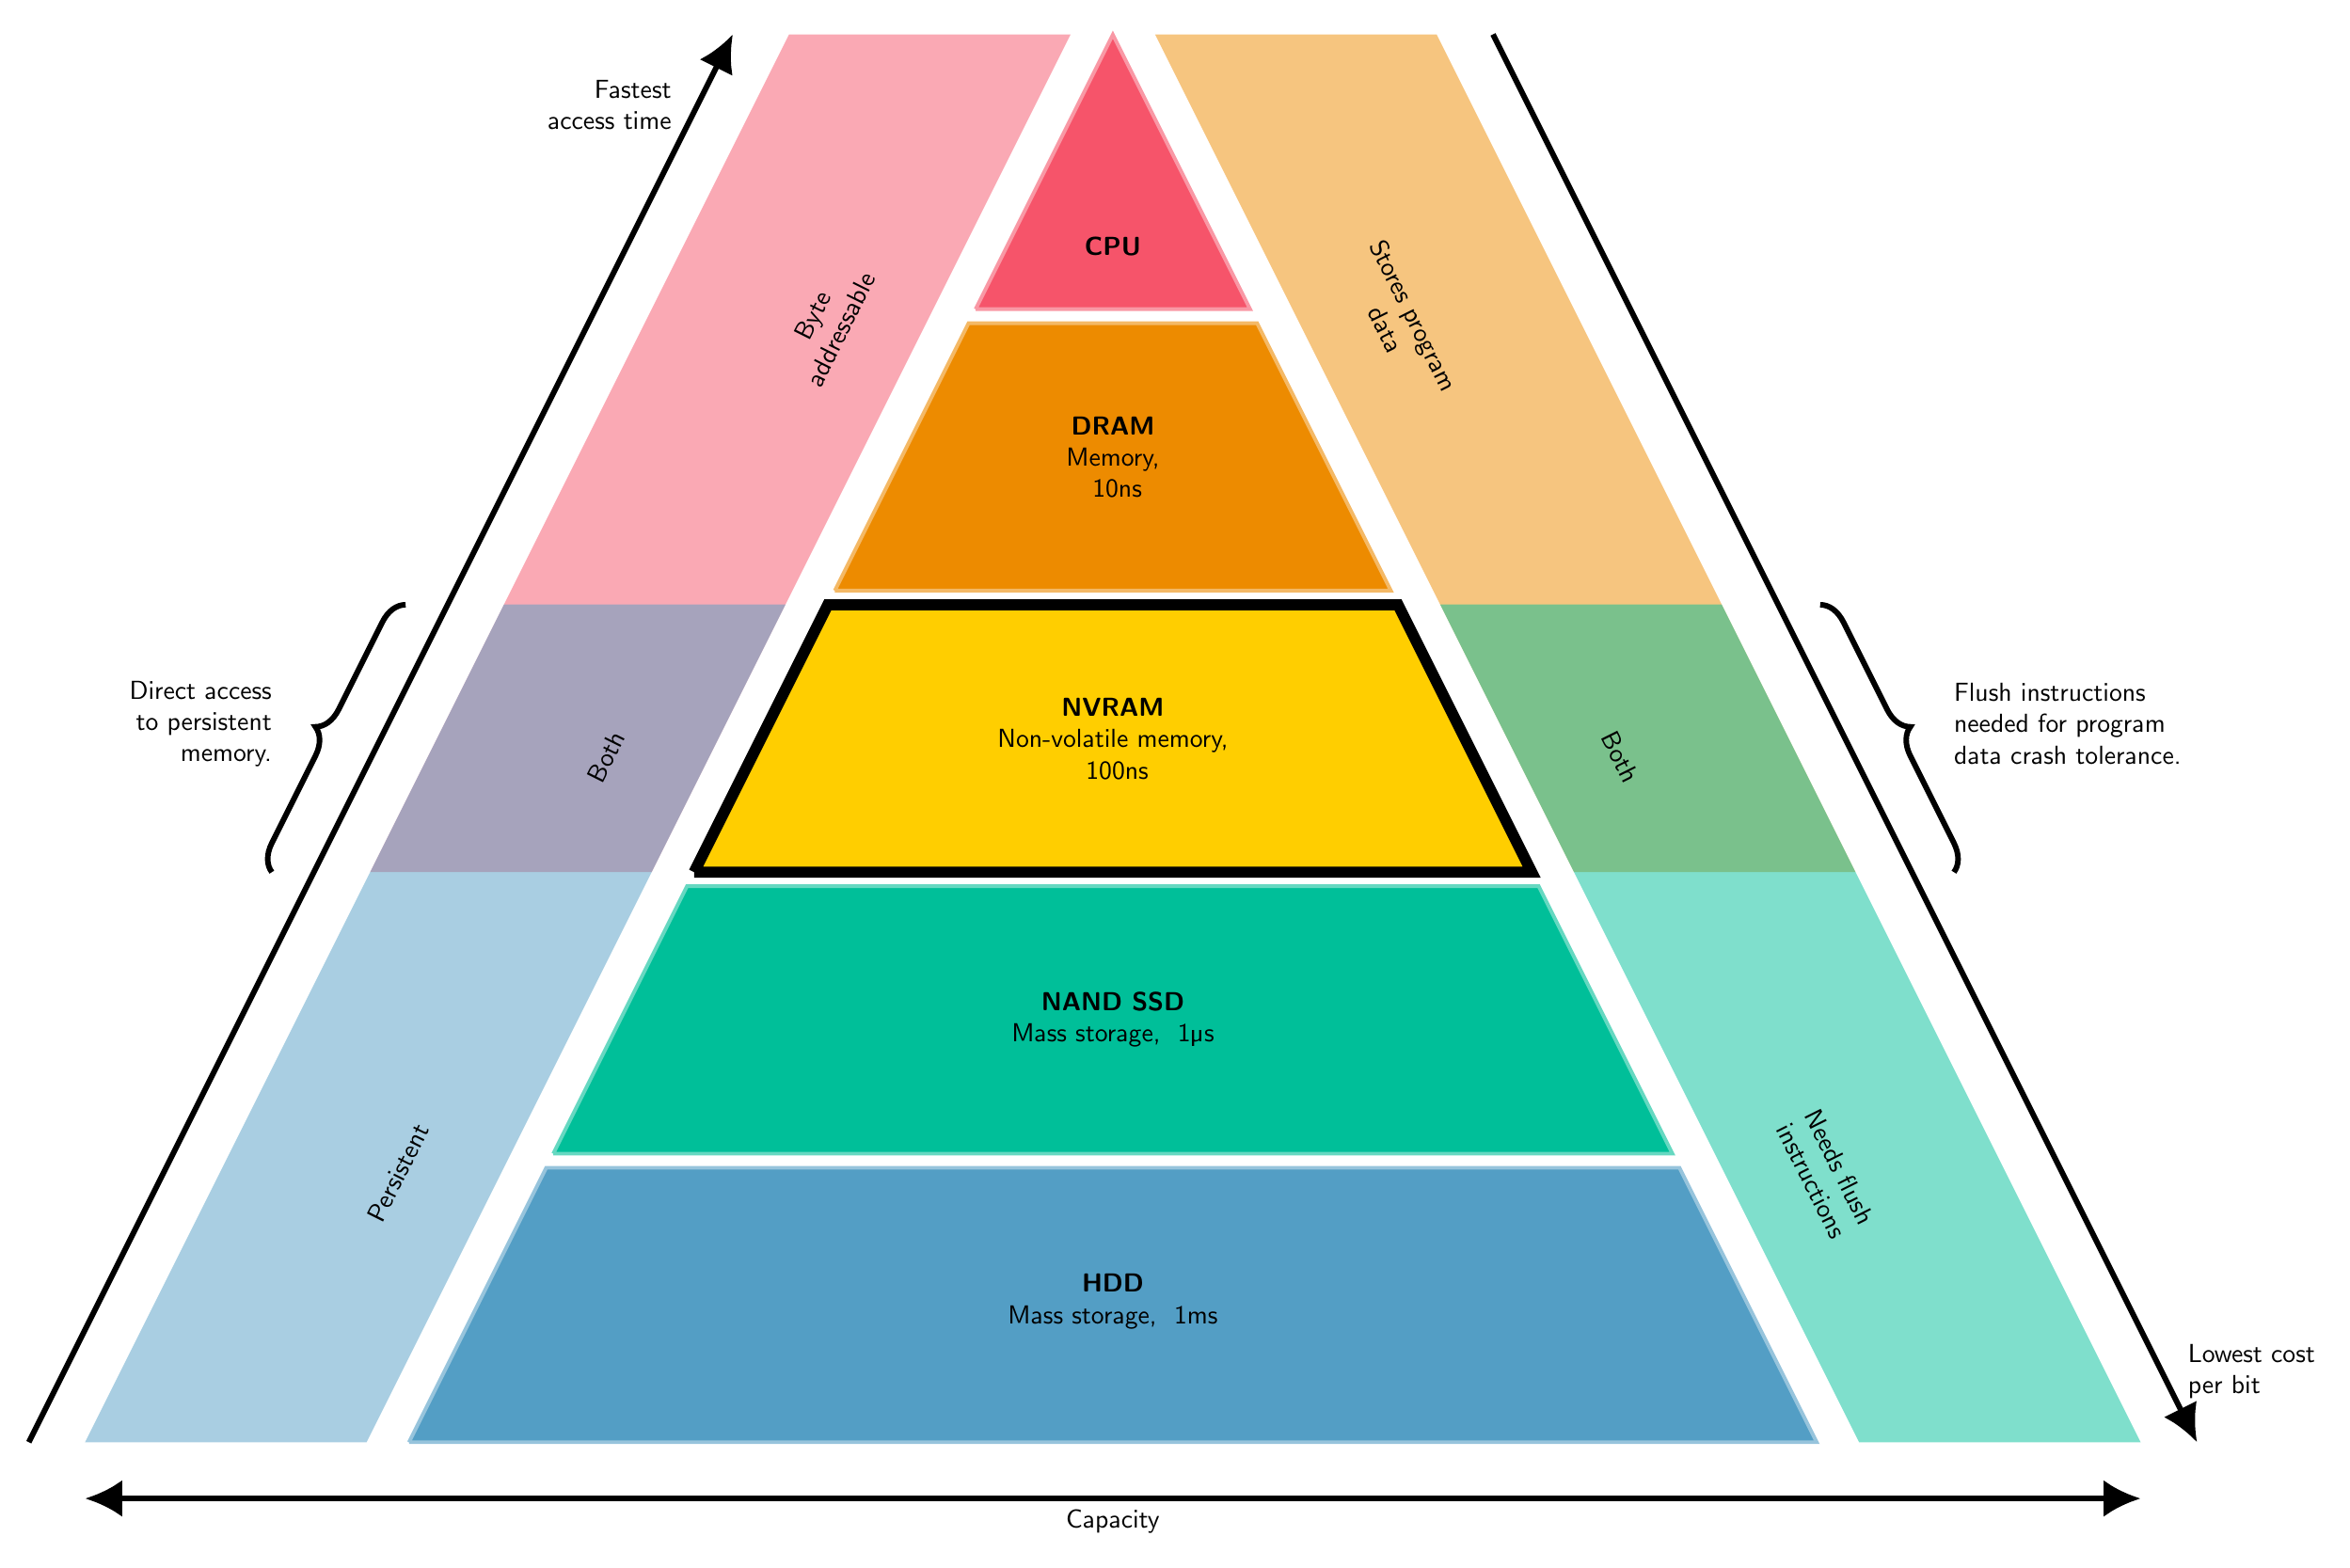
\begin{tikzpicture}[scale=1.9]
        \tikzstyle{every node}=[font=\normalsize]
        \definecolor{myblue}{RGB}{83,158,197}
        \definecolor{mylightblue}{RGB}{151,196,220}
        \definecolor{mygreen}{RGB}{0,191,153}
        \definecolor{mylightgreen}{RGB}{102,216,193}
        \definecolor{myyellow}{RGB}{255,206,0}
        \definecolor{mylightyellow}{RGB}{255,230,127}
        \definecolor{myorange}{RGB}{237,139,0}
        \definecolor{mylightorange}{RGB}{244,185,102}
        \definecolor{myred}{RGB}{246,84,106}
        \definecolor{mylightred}{RGB}{249,152,165}
        \node (a1) at (-5, 0) {};
        \node (a2) at (5, 0) {};
        \node (a3) at (-4.025, 1.95) {};
        \node (a4) at ( 4.025, 1.95) {};
        \draw[mylightblue, fill=myblue, line width=0.5mm] (a1.center) -- (a2.center) -- (a4.center) -- (a3.center) -- (a1.center);
        \node[align=center] (a5) at (0, 1) {\textbf{HDD}\\Mass storage, ~1ms};
        \node (b1) at (-3.975, 2.05) {};
        \node (b2) at ( 3.975, 2.05) {};
        \node (b3) at (-3.025, 3.95) {};
        \node (b4) at ( 3.025, 3.95) {};
        \draw[mylightgreen, fill=mygreen, line width=0.5mm] (b1.center) -- (b2.center) -- (b4.center) -- (b3.center) -- (b1.center);
        \node[align=center] (b5) at (0, 3) {\textbf{NAND SSD}\\Mass storage, ~1µs};
        \node (c1) at (-2.975, 4.05) {};
        \node (c2) at ( 2.975, 4.05) {};
        \node (c3) at (-2.025, 5.95) {};
        \node (c4) at ( 2.025, 5.95) {};
        \draw[black, fill=myyellow, line width=1.5mm] (c1.center) -- (c2.center) -- (c4.center) -- (c3.center) -- (c1.center);
        \node[align=center] (c5) at (0, 5) {\textbf{NVRAM}\\Non-volatile memory,\\~100ns};
        \node (d1) at (-1.975, 6.05) {};
        \node (d2) at ( 1.975, 6.05) {};
        \node (d3) at (-1.025, 7.95) {};
        \node (d4) at ( 1.025, 7.95) {};
        \draw[mylightorange, fill=myorange, line width=0.5mm] (d1.center) -- (d2.center) -- (d4.center) -- (d3.center) -- (d1.center);
        \node[align=center] (d5) at (0, 7) {\textbf{DRAM}\\Memory,\\~10ns};
        \node (e1) at (-0.975, 8.05) {};
        \node (e2) at ( 0.975, 8.05) {};
        \node (e3) at (0, 10) {};
        \draw[mylightred, fill=myred, line width=0.5mm] (e1.center) -- (e2.center) -- (e3.center) -- (e1.center);
        \node[align=center] (e4) at (0, 8.5) {\textbf{CPU}};
        \node (g1) at ([xshift = -0.3cm] e3.center) {};
        \node (g2) at ([xshift = -2.3cm] e3.center) {};
        \node (g3) at ([xshift = -2.3cm] c1.center) {};
        \node (g4) at ([xshift = -0.3cm] c1.center) {};
        \draw[myred, fill=myred, fill opacity = 0.5, draw opacity = 0] (g1.center) -- (g2.center) -- (g3.center) -- (g4.center) -- (g1.center);
        \node (h1) at ([xshift = -0.3cm] c3.center) {};
        \node (h2) at ([xshift = -2.3cm] c3.center) {};
        \node (h3) at ([xshift = -2.3cm] a1.center) {};
        \node (h4) at ([xshift = -0.3cm] a1.center) {};
        \draw[myblue, fill=myblue, fill opacity = 0.5, draw opacity = 0] (h1.center) -- (h2.center) -- (h3.center) -- (h4.center) -- (h1.center);

        \draw[draw opacity = 0] ([xshift = -0.3] d1.center) -- ([xshift = -0.3] e3.center) node [midway, above, sloped, anchor = south, xshift = -1cm, yshift = 1.25cm, text width = 3cm, align = center] {Byte\\addressable};
        \draw[draw opacity = 0] ([xshift = -0.3] a1.center) -- ([xshift = -0.3] b3.center) node [midway, above, sloped, anchor = south, xshift = -1cm, yshift = 1.5cm, text width = 3cm, align = center] {Persistent};
        \draw[draw opacity = 0] ([xshift = -0.3] c1.center) -- ([xshift = -0.3] c3.center) node [midway, above, sloped, anchor = south, xshift = -1.15cm, yshift = 1.5cm, text width = 3cm, align = center] {Both};

        \draw[decorate, decoration = {brace, amplitude = 10pt}, black, line width = 0.75mm] ([xshift = -3cm] c1.center) -- ([xshift = -3cm] c3.center) node [midway, xshift = -0.75cm, yshift=0.2cm, anchor = east, align = right] {Direct access\\to persistent\\memory.};

        
        \node (i1) at ([xshift = 0.3cm] e3.center) {};
        \node (i2) at ([xshift = 2.3cm] e3.center) {};
        \node (i3) at ([xshift = 2.3cm] c2.center) {};
        \node (i4) at ([xshift = 0.3cm] c2.center) {};
        \draw[myorange, fill=myorange, fill opacity = 0.5, draw opacity = 0] (i1.center) -- (i2.center) -- (i3.center) -- (i4.center) -- (i1.center);
        \node (j1) at ([xshift = 0.3cm] c4.center) {};
        \node (j2) at ([xshift = 2.3cm] c4.center) {};
        \node (j3) at ([xshift = 2.3cm] a2.center) {};
        \node (j4) at ([xshift = 0.3cm] a2.center) {};
        \draw[mygreen, fill=mygreen, fill opacity = 0.5, draw opacity = 0] (j1.center) -- (j2.center) -- (j3.center) -- (j4.center) -- (j1.center);

        \draw[draw opacity = 0] ([xshift = 0.3] d2.center) -- ([xshift = 0.3] e3.center) node [midway, above, sloped, anchor = south, xshift = 1cm, yshift = 1.25cm, text width = 7cm, align = center] {Stores program\\data};
        \draw[draw opacity = 0] ([xshift = 0.3] a2.center) -- ([xshift = 0.3] b4.center) node [midway, above, sloped, anchor = south, xshift = 1cm, yshift = 1.25cm, text width = 6cm, align = center] {Needs flush\\instructions};
        \draw[draw opacity = 0] ([xshift = 0.3] c2.center) -- ([xshift = 0.3] c4.center) node [midway, above, sloped, anchor = south, xshift = 1.15cm, yshift = 1.5cm, text width = 3cm, align = center] {Both};

        \draw[decorate, decoration = {brace, amplitude = 10pt, mirror}, black, line width = 0.75mm] ([xshift = 3cm] c2.center) -- ([xshift = 3cm] c4.center) node [midway, xshift = 0.75cm, yshift=0.2cm, anchor = west, align = left] {Flush instructions\\needed for program\\data crash tolerance.};

        
        \path [-{Latex[length=5mm,width=5mm]}, line width=0.75mm] ([xshift=-0.4cm]h3.center) edge node[pos = 0.95, anchor = east, align = right, xshift=-0.2cm] {Fastest\\access time} ([xshift=-0.4cm]g2.center);
        \path [-{Latex[length=5mm,width=5mm]}, line width=0.75mm] ([xshift=0.4cm]i2.center) edge node[pos = 0.95, anchor = west, align = left, xshift=0.2cm] {Lowest cost\\per bit} ([xshift=0.4cm]j3.center);
        \path [{Latex[length=5mm,width=5mm]}-{Latex[length=5mm,width=5mm]}, line width=0.75mm] ([yshift=-0.4cm]h3.center) edge node[sloped, anchor=center, below] {Capacity} ([yshift=-0.4cm]j3.center);
        

      \end{tikzpicture}
    \end{tikzfigure}
  }

  \block{Immutable structures as an alternative to journals}{
    % Linked list node
    \newcommand\LLNode[4]{
      \node[draw, line width=1mm, minimum height = 15mm, minimum width = 15mm, #4, text = black, fill = #4!25!white] at (#1) (#2block) {#3};
      \node[draw, line width=1mm, minimum height = 5mm, minimum width = 15mm, anchor = north, #4, fill = #4!15!white] at ([yshift=\pgflinewidth]#2block.south) (#2ptr) {};
    }
    \newcommand\LLNodeH[4]{
      \node[draw, line width=1mm, minimum height = 15mm, minimum width = 15mm, #4, text = black, fill = #4!25!white] at (#1) (#2block) {#3};
      \node[draw, line width=1mm, minimum height = 15mm, anchor = west, #4, fill = #4!15!white] at ([xshift=-\pgflinewidth]#2block.east) (#2ptr) {};
    }

    \centering Linked List ``ACD'' $\rightarrow$ ``ABCD''.
    \vspace{2em}

    \begin{minipage}{0.48\linewidth}
      \centering \textbf{Transaction journals}
      \begin{tikzfigure}[An example of a linked list to which a node is added after the head. The persistency is secured through a transactionnal journal.\par]        
        \begin{tikzpicture}
          \LLNode{0,0}{b0}{A}{black!50!green};
          \LLNode{0,-3}{a1}{B}{black!50!green};
          \LLNode{0,-6}{b1}{C}{red};
          \LLNode{0,-9}{b2}{D}{red};

          \node[draw, line width = 1mm, minimum width = 5cm] at ([xshift = 8cm]b0block.center) (j0) {Journal};
          \node[draw, line width = 1mm, minimum width = 5cm, anchor = north] at ([yshift = \pgflinewidth]j0.south) (j1) { \dots };
          \node[draw, line width = 1mm, minimum width = 5cm, anchor = north, minimum height = 3cm] at ([yshift = \pgflinewidth]j1.south) (j5) {  };
          \node[draw, line width = 1mm, minimum width = 5cm, anchor = north, minimum height = 3cm] at ([yshift = \pgflinewidth]j5.south) (j2) {  };
          \node[draw, line width = 1mm, minimum width = 5cm, anchor = north] at ([yshift = \pgflinewidth]j2.south) (j4) { \dots };
          
          \LLNode{[yshift = 0.35cm]j2.center}{j3}{A}{red};
          
          \path[draw, -{Latex[length=5mm,width=5mm]}, line width=1mm] (b0ptr.center) -- (a1block.north);
          \path[draw, -{Latex[length=5mm,width=5mm]}, line width=1mm] (a1ptr.center) -- (b1block.north);
          \path[draw, -{Latex[length=5mm,width=5mm]}, line width=1mm] (b1ptr.center) -- (b2block.north);
          \path[draw, -{Latex[length=5mm,width=5mm]}, line width=1mm] (j3ptr.center) -| ([xshift = 3cm]b1block.east) -- (b1block.east);
          
          \path[draw, -{Rays}, line width=1mm] (b2ptr.center) -- ([yshift=-1cm]b2ptr.center);
          \path[draw, dashed, -{Latex[length=5mm,width=5mm]}, line width = 1mm] (j2.west) -- (b0block.east);
          \node[align = center] at (j5.center) {\small Allocation\\\small(16B)};
          \path[draw, dashed, -{Latex[length=5mm,width=5mm]}, line width = 1mm] (j5.west) -- (a1block.east);
          
        \end{tikzpicture}
      \end{tikzfigure}

    \end{minipage}
    \hfill
    \begin{minipage}{0.48\linewidth}
      \centering \textbf{Immutable data structures}
      \begin{tikzfigure}[The same operation, now with an immutable approach to the linked list.\par]        
        \begin{tikzpicture}
          \LLNodeH{0,0}{b0}{A}{red};
          \LLNodeH{6,0}{b1}{C}{red};
          \LLNodeH{9,0}{b2}{D}{red};
          \LLNodeH{0,3}{a0}{A}{black!50!green};
          \LLNodeH{3,3}{a1}{B}{black!50!green};

          \node[anchor = east] at ([xshift=-0.5cm] b0block.west) {Original};
          \node[anchor = east] at ([xshift=-0.5cm] a0block.west) {New};
          
          \path[draw, -{Latex[length=5mm,width=5mm]}, line width=1mm] (b0ptr.center) -- (b1block.west);
          \path[draw, -{Latex[length=5mm,width=5mm]}, line width=1mm] (b1ptr.center) -- (b2block.west);
          \path[draw, -{Latex[length=5mm,width=5mm]}, line width=1mm] (a0ptr.center) -- (a1block.west);
          \path[draw, -{Latex[length=5mm,width=5mm]}, line width=1mm] (a1ptr.center) -| (b1block.north);
          \path[draw, -{Rays}, line width=1mm] (b2ptr.center) -- ([xshift=2cm]b2ptr.center);

          \path (0, -4.5);
          \path (0,  7.5);
        \end{tikzpicture}
      \end{tikzfigure}

    \end{minipage}
  }
  
  \block{Rust, a systems programming language}{
    \begin{minipage}{0.48\linewidth}
      \inputminted[autogobble]{rust}{showcase.rs}
    \end{minipage}
    \hfill
    \begin{minipage}{0.48\linewidth}
      \begin{itemize}
      \item Mutability control
      \item Overload operators (\texttt{Deref}).
      \item Manage heap allocation.
      \end{itemize}
    \end{minipage}
  }
  \block{Our goal}{
    \centering Create a user-friendly, performant and innovative transactionnal persistent memory library in Rust, using immutable data structures to avoid journals.
  }
  
  \column{0.5}
  \block{A single-threaded persistent memory allocator}{
    Memory block figure, with all the situations we can encounter
  }
  \block{Persistent Rust standard library types}{
    PBox, PVec, and how they work (copy when deref mut), with figure
  }
  \block{A persistent Hitchhiker Tree data structure}{
    A figure with a small tree and little text that says we have the two (std and nvram) versions?
  }
  \block{Interior mutability in a persistent context}{
    How we use HHTree to allow interior mutability and keep tree-like topology transparently for the user
  }
  
\end{columns}
\end{document}
